\chapter{Implementation}
This chapter is concerned with the implementation details of the individidual components introduced in Chapter \ref{chapter:4}. This includes the development of the Unity application responsible for producing a video stream from the front-facing camera of the Hololens, the development of the human detection and direction system, as well as the reactive control systems implemented on ARTA. Previous work in the PRL had utilized the Hololens camera to capture images that were then processed on an external computer, but where this project differs is that a video stream was required to be able to perform real-time object detection. As such, a large amount of time was spent at the very beginning of the project trying to produce a video stream, since the whole project depended on this form of visual input.

\begin{figure}[ht]
	\centering
	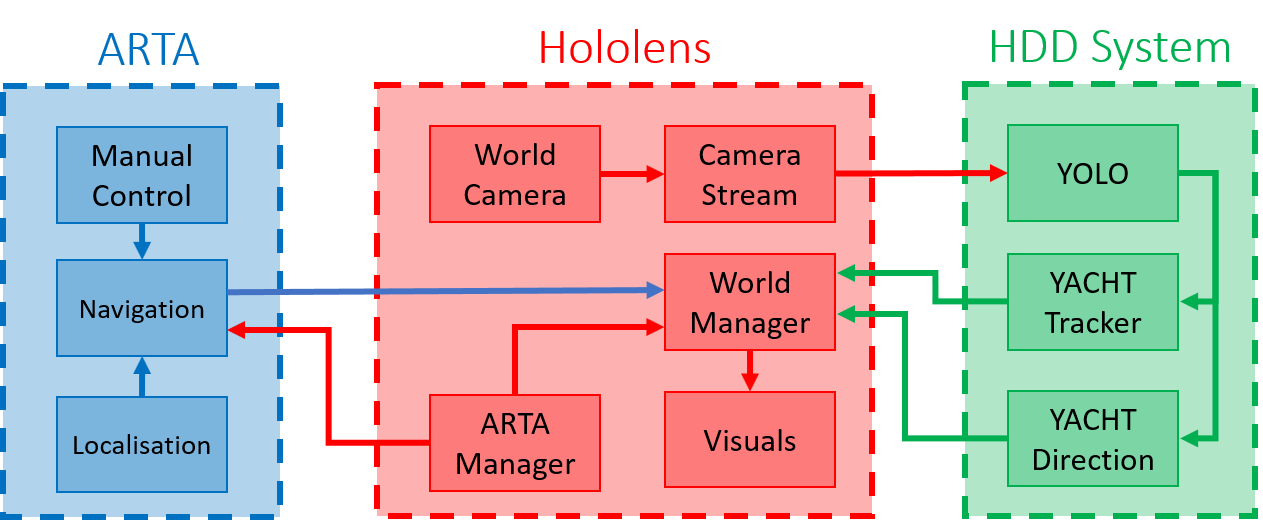
\includegraphics[width=1.0\linewidth]{img/chapter5_implementation/detailedSystemDiagram.png}
	\caption{System diagram detailing individual components}
	\label{fig:detailedHL}
\end{figure}